\chapter{Methods and procedures} \label{ch:methods}

In this section I outline the methods for actually extracting homology information, \ie~Betti numbers, from images generated by simulating the Gray-Scott system. \refSect{sec:thresholding} describes the process of preparing the images for computation and the considerations and problems that arise. \refSect{sect:entropy} is concerned with calculating the entropy of the system given the homological data. \refsect{ch1:gs-simulation} details the conditions for generating the pattern images.

\section{Obtaining Betti numbers}

Given the complicated overview of cubical homology theory given in \refsect{ch2:cubicalhomology}, one might expect extracting the Betti numbers from an image to be a difficult undertaking. Fortunately, homology software developed at Rutgers, with contributions from Georgia Tech and Konstantin Mischaikow (Mathematics '79), titled \textsc{CHomP}, (Computational Homology Project), facilitates this process\rf{chomp}. Furthermore, the way it works is extremely intuitive, essentially counting clusters of adjacent pixels. This requires a 2-bit binary image as input.\footnote{That is, an image with \emph{only} black and white pixels.} Since the images output by the Gray-Scott simulation are greyscale, they must first be converted to a 2-bit image

\subsection{Thresholding} \label{sect:thresholding}

The output of the Gray-Scott simulation is a series of 8-bit greyscale images, \ie~there are 256 possible shades of grey (0 is black, 255 is white). The color map is such that $V_{min} = 0.0 \rightarrow 255$ and $V_{max} = 0.4 \rightarrow 0$. In other words, white and black indicate low and high concentration of $V$ respectively\footnote{$V_{max}$ was chosen based on the average maximum of $V \approx 0.4$ for all the patterns examined.}. Each image is thresholded at some value $T \in [0,255]$. That is, all pixels with intensity $< T$ are now black and those with intensity $> T$ are now white.

\begin{sidewaysfigure}[hp]
	\centering
	\begin{subfigure}[b]{0.45\textwidth}
                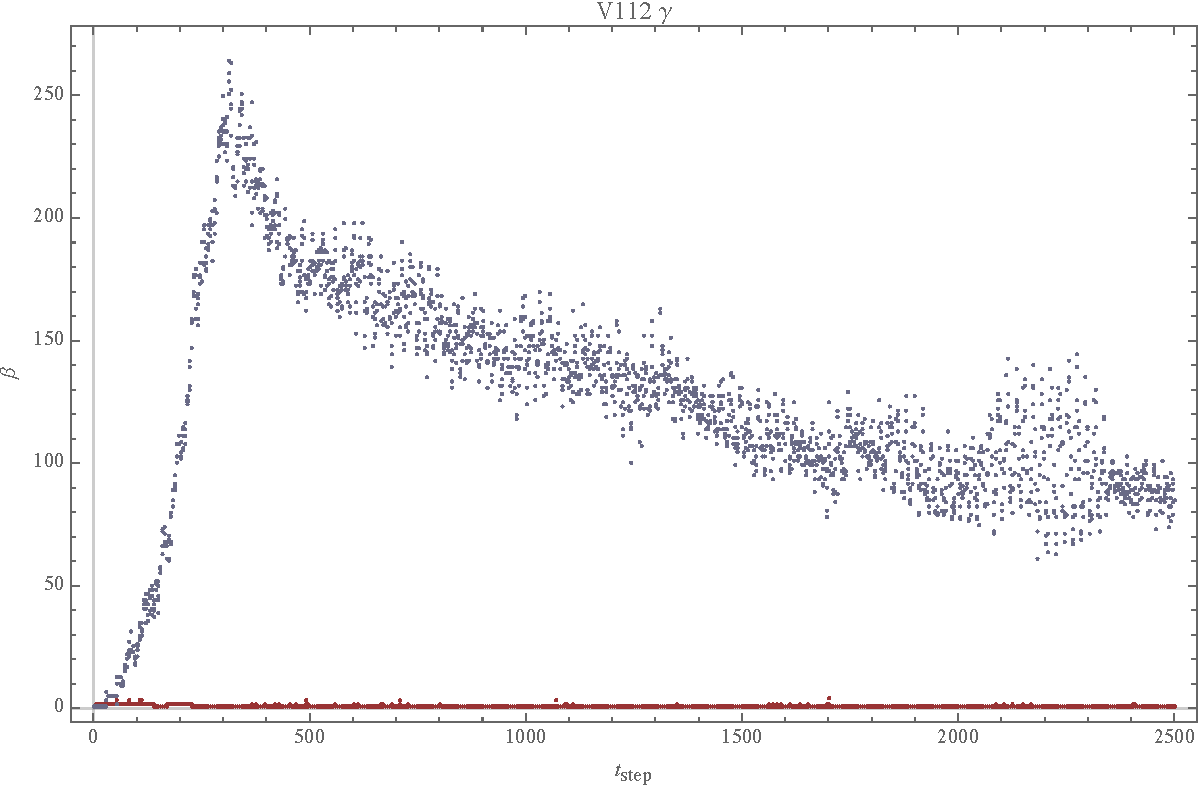
\includegraphics[width=\textwidth]{bplot_gamma112}
                \caption{$\gamma$, $T = 112$.}
                \label{fig:bplot_gamma112}
        \end{subfigure} \quad
	\begin{subfigure}[b]{0.45\textwidth}
                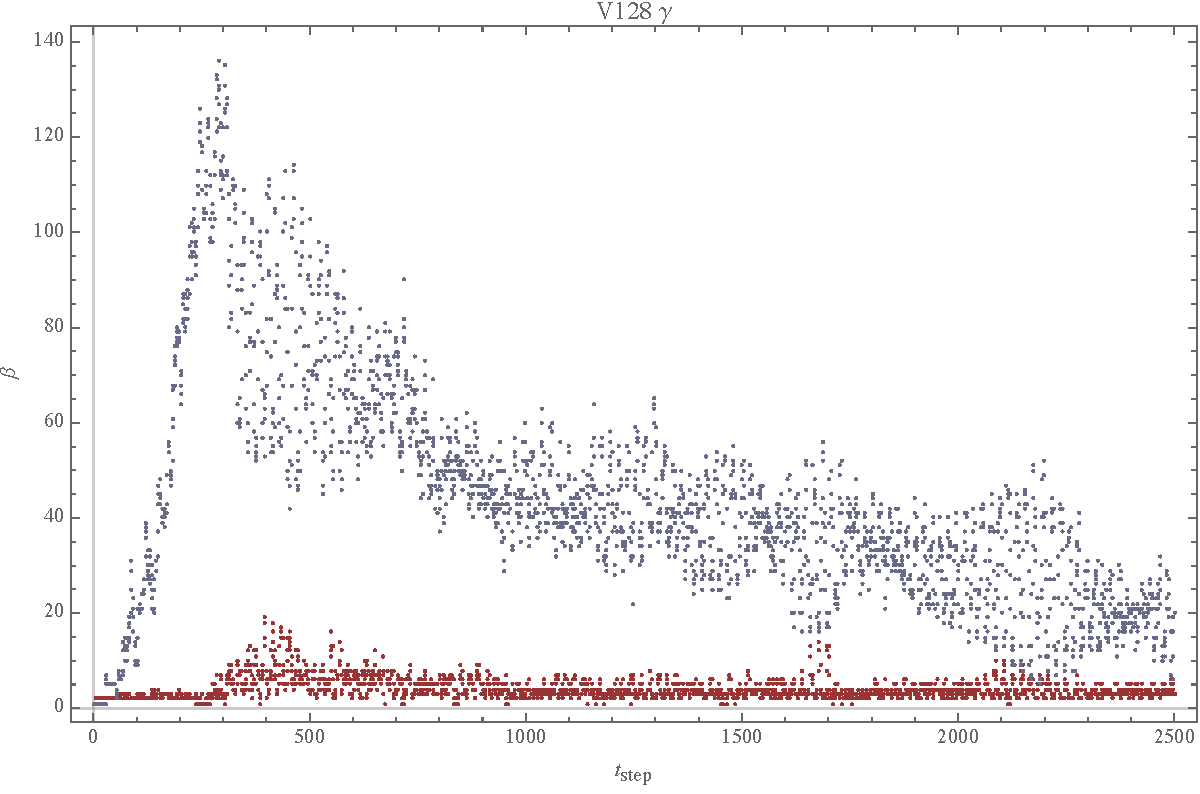
\includegraphics[width=\textwidth]{bplot_gamma128}
                \caption{$\gamma$, $T = 128$.}
                \label{fig:bplot_gamma128}
        \end{subfigure} \hfill \\
        %
	\begin{subfigure}[b]{0.45\textwidth}
                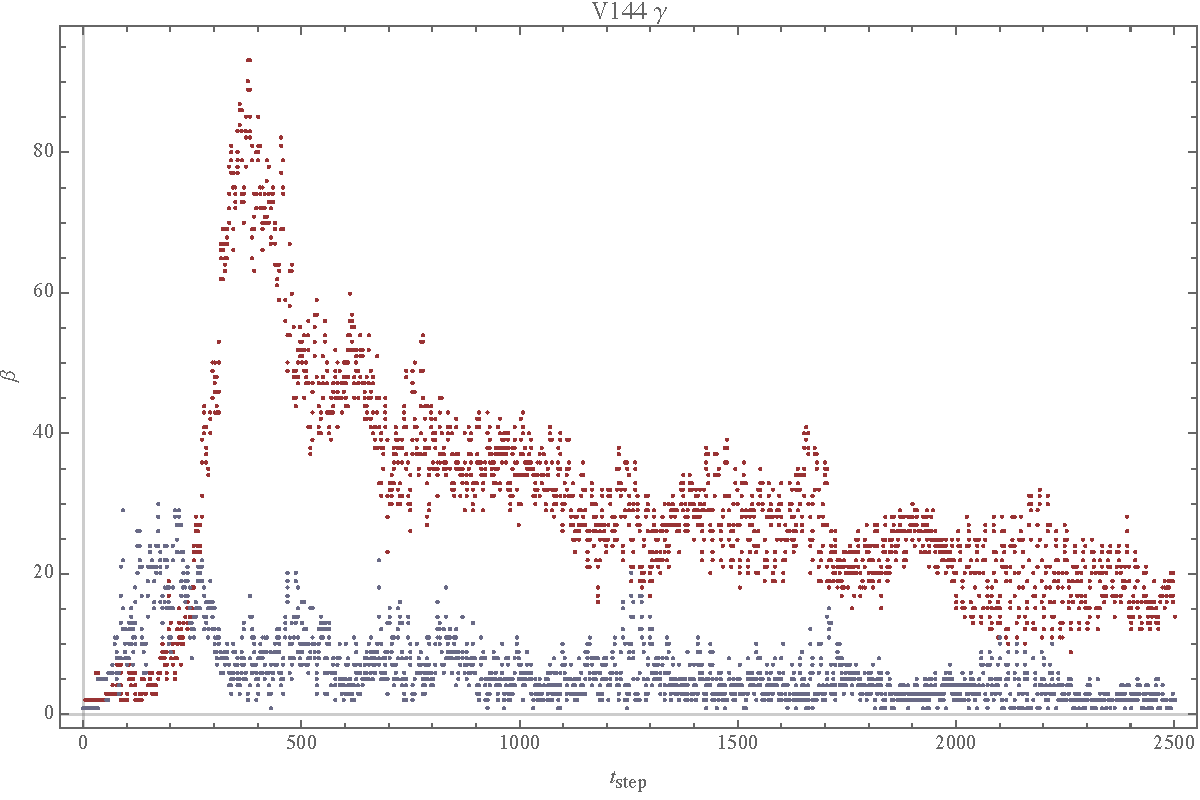
\includegraphics[width=\textwidth]{bplot_gamma144}
                \caption{$\gamma$, $T = 144$.}
                \label{fig:bplot_gamma144}
       \end{subfigure} \quad
       \begin{subfigure}[b]{0.45\textwidth}
                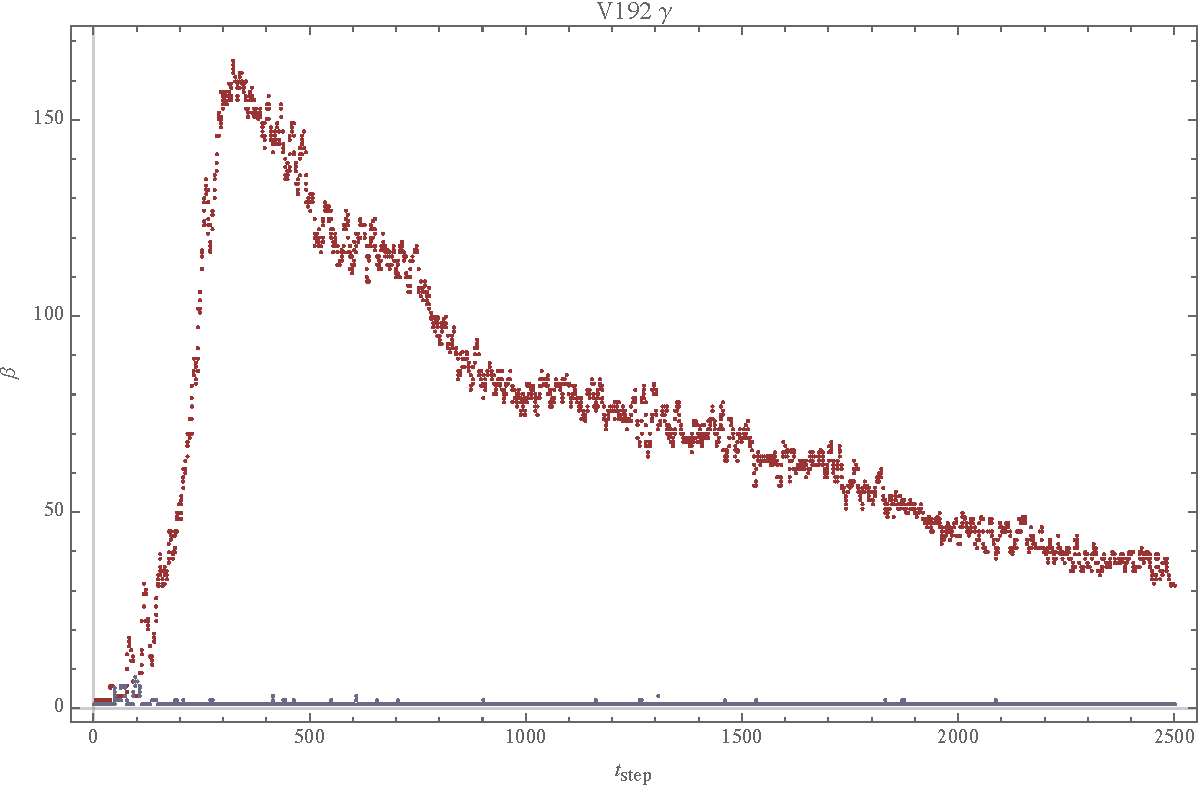
\includegraphics[width=\textwidth]{bplot_gamma192}
                \caption{$\gamma$, $T = 192$.}
                \label{fig:bplot_gamma192}
        \end{subfigure}
        
        \caption{A plot of the time series of Betti numbers for pattern $\gamma$. The zeroth Betti number $\beta_0$ is shown in red and the first Betti number $\beta_1$ shown in blue. Different thresholds $T =$ 112, 128, 144, and 192 demonstrate the dramatic effect of thresholding for some patterns. For very high and low $T$, the image loses any resemblance to the original image. Slightly varying the threshold, however, can reduce the amount of ``noise'' in the data.} \label{fig:bplots_gamma}
\end{sidewaysfigure}

A logical choice for $T$ is the median pixel intensity of the image\rf{krishan_2007}. But, in the case of sparse patterns like $\alpha$ and $\epsilon$ (\refFigs{fig:alpha_sample}{fig:epsilon_sample} respectively), this results in a completely black image since the median is very high. Although other adaptive methods of thresholding exist\rf{mischaikow_2002}, the definitive answer to thresholding problems is \emph{persistent homology}, which is a large leap in terms of complexity\rf{persistence_2008}. This approach is concerned with the ``birth'' and ``death'' of homology components as the threshold is varied in a away that circumvents the need for a threshold altogether. Persistent homology has seen great success in analyzing large sets of nonlinear data\rf{weinberger_2011}.

\begin{figure}[h]
	\centering
	\begin{subfigure}[b]{0.33\textwidth}
                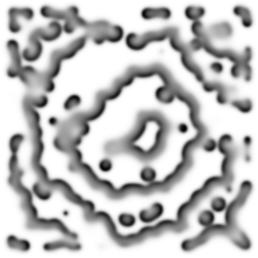
\includegraphics[width=\textwidth]{spiral_b0-5_b1-32.png}
                \caption{}
                \label{fig:spiral_grey}
        \end{subfigure} \quad
	\begin{subfigure}[b]{0.33\textwidth}
                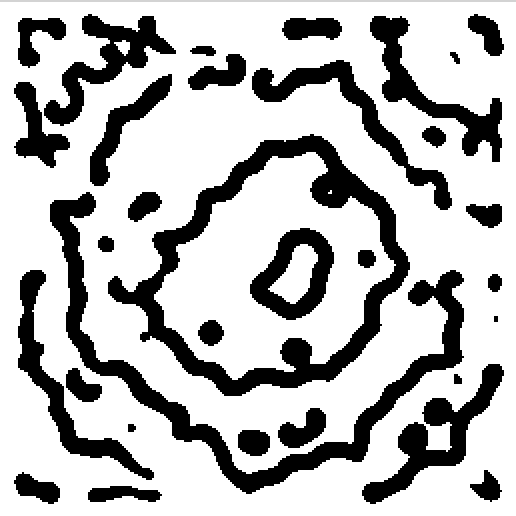
\includegraphics[width=\textwidth]{spiral_144.png}
                \caption{}
                \label{fig:spiral_144}
        \end{subfigure}
        \caption{On the left is the spiral pattern with $(F, k) = (0.035, 0.060)$ while the figure on the right shows the pattern thresholded at $T = 144$. The Betti numbers for this pattern are $\beta_0 = 32$, $\beta_1 = 5$.}
        \label{fig:spiral_thresh}
\end{figure}

Short of persistent homology, another reasonable choice would be to split right down the middle, $T = 128$, but as \refFigs{fig:bplots_gamma}{fig:thresholds} illustrate, some information is lost in the process. Thus the optimal choice of threshold depends entirely on the characteristics of that image. The patterns produced by the Gray-Scott system are varied and no single value of $T$ is ideal for all $(F, k)$, but experimentally, slightly higher $T$ better agrees with the characteristics of the original pattern. For this reason, the value $T = 144$ was chosen to perform the all the calculations.

Provided in the \textsc{CHomP} software package is a method for simply thresholding images, \texttt{chomp-greyscale-to-cubical} (which takes a single image input, at threshold, and an output filename). The output is a text file which contains the coordinates of white pixels. This is what is then analyzed to produce Betti numbers. A script automates this process for all 2,500 \texttt{png} files generated by the simulation (see \refSect{ch1:gs-simulation}).

\begin{figure}[pt]
	\centering
	\begin{subfigure}[b]{0.25\textwidth}
                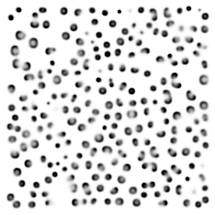
\includegraphics[width=\textwidth]{alpha_v_grey.png}
                \caption{$\alpha$ in greyscale.}
                \label{fig:alpha_grey}
        \end{subfigure} \quad
	\begin{subfigure}[b]{0.25\textwidth}
                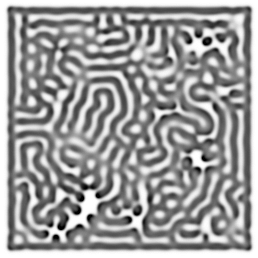
\includegraphics[width=\textwidth]{gamma_v_grey.png}
                \caption{$\gamma$ in greyscale.}
                \label{fig:gamma_grey}
        \end{subfigure}\quad
	\begin{subfigure}[b]{0.25\textwidth}
                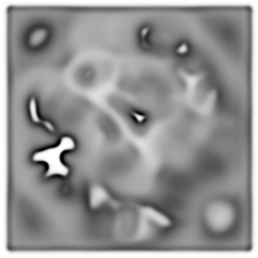
\includegraphics[width=\textwidth]{beta_v_grey.png}
                \caption{$\beta$ in greyscale.}
                \label{fig:beta_grey}
        \end{subfigure}\hfill \\
        ~ %add desired spacing between images, e. g. ~, \quad, \qquad, \hfill etc.
          %(or a blank line to force the subfigure onto a new line)
	\begin{subfigure}[b]{0.25\textwidth}
                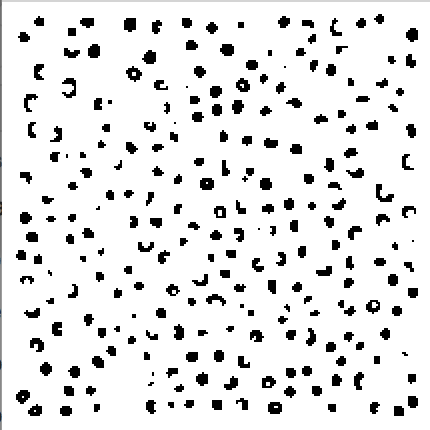
\includegraphics[width=\textwidth]{alpha_v_thresh112.png}
                \caption{$\alpha$, $T =$ 112.}
                \label{fig:alpha_112}
        \end{subfigure} \quad
	\begin{subfigure}[b]{0.25\textwidth}
                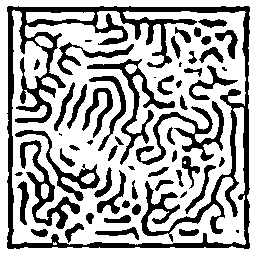
\includegraphics[width=\textwidth]{gamma_thresh112.png}
                \caption{$\gamma$, $T =$ 112.}
                \label{fig:gamma_112}
        \end{subfigure}\quad
        \begin{subfigure}[b]{0.25\textwidth}
                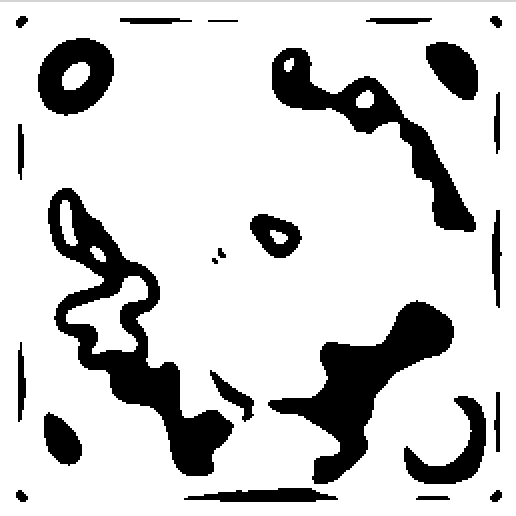
\includegraphics[width=\textwidth]{beta_v_thresh112.png}
                \caption{$\beta$, $T =$ 112.}
                \label{fig:beta_112}
        \end{subfigure} \hfill \\
        
        \begin{subfigure}[b]{0.25\textwidth}
                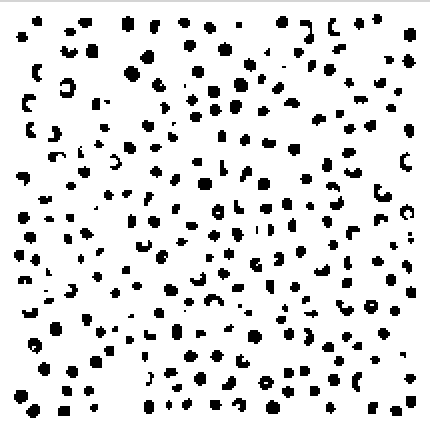
\includegraphics[width=\textwidth]{alpha_v_thresh128.png}
                \caption{$\alpha$, $T =$ 128.}
                \label{fig:alpha_128}
        \end{subfigure} \quad
         \begin{subfigure}[b]{0.25\textwidth}
                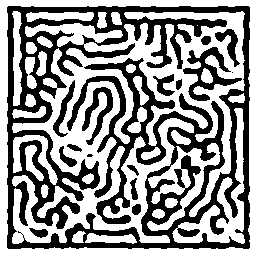
\includegraphics[width=\textwidth]{gamma_thresh128.png}
                \caption{$\gamma$, $T =$ 128.}
                \label{fig:gamma_128}
        \end{subfigure}\quad
        \begin{subfigure}[b]{0.25\textwidth}
                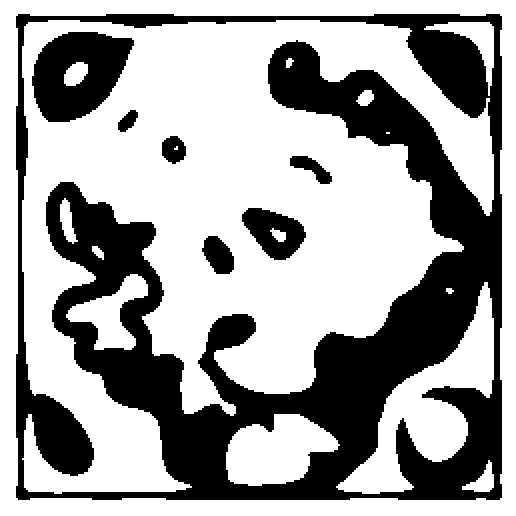
\includegraphics[width=\textwidth]{beta_v_thresh128.png}
                \caption{$\beta$, $T =$ 128.}
                \label{fig:beta_144}
        \end{subfigure} \hfill \\
        
        \begin{subfigure}[b]{0.25\textwidth}
                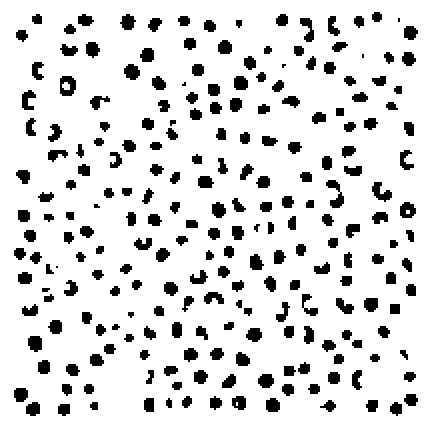
\includegraphics[width=\textwidth]{alpha_v_thresh144.png}
                \caption{$\alpha$, $T =$ 144.}
                \label{fig:alpha_144}
        \end{subfigure} \quad
         \begin{subfigure}[b]{0.25\textwidth}
                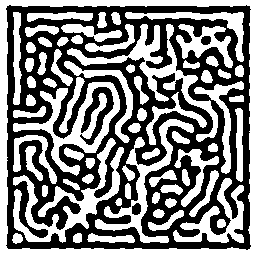
\includegraphics[width=\textwidth]{gamma_thresh144.png}
                \caption{$\gamma$, $T =$ 144.}
                \label{fig:gamma_144}
        \end{subfigure} \quad
         \begin{subfigure}[b]{0.25\textwidth}
                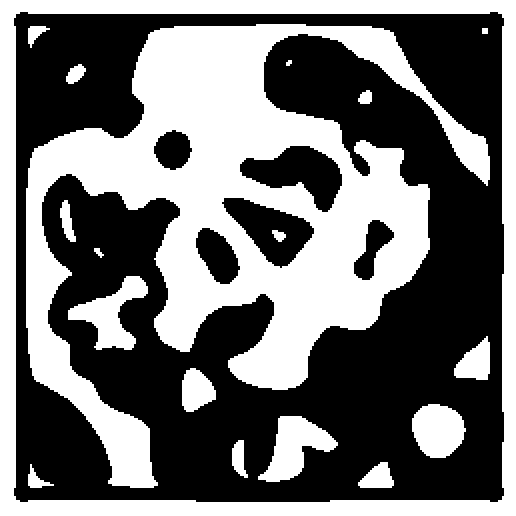
\includegraphics[width=\textwidth]{beta_v_thresh144.png}
                \caption{$\beta$, $T =$ 144.}
                \label{fig:beta_144}
        \end{subfigure} \hfill
        \caption{Patterns $\alpha$, $\gamma$, and $\beta$ at various thresholds. Some features of less stable patterns such as $\gamma$ and $\beta$ are lost when thresholded. Slightly higher thresholds ($>128$) tend to capture the topology of the original pattern better.}\label{fig:thresholds}
\end{figure}

\subsection{Performing cubical homology} \label{sect:chomping}

Once the images are thresholded at some value, the \textsc{CHomP} method \texttt{chomp-cubical} analyzes and returns Betti numbers $\beta_0$, $\beta_1$, and $\beta_2$.  A single calculation of Betti numbers takes about 1-3s on a 4.2 GHz Intel i7 processor. This process is performed for each of 2,500 text files produced by \texttt{chomp-greyscale-to-cubical} to generate a single CSV file of the Betti numbers $\beta_0$, $\beta_1$, and $\beta_2$ for each time step.\footnote{The Betti number $\beta_2$ is included only for posterity; $\beta_2$ = 0 for all time steps.}

\subsection{Calculating entropy} \label{sect:entropy}

In physics, entropy usually denotes the amount of ``disorder'' of a system. Shannon's entropy, $S(X)$, indicates the average amount of information that an observer gains \emph{after} receiving a realized outcome $x$ of the random variable $X$\rf{grunwald_2004}. We wish to use homology information to provide a sense of how predictable (how complex) the Gray-Scott system is for a given choice of parameters (namely $F, k$). In general, the Shannon entropy $S$ of some variable $X$ with possible values $\{ x_1, \ldots, x_N \}$ and probability distribution $P(x_i) = P_i$ is defined by
\begin{align} \label{eq:shannon}
	S(X) = - \sum_{i=1}^{N} P_i \log{ P_i}.
\end{align}
In our case, the Shannon entropy gives a picture of the average minimum number of states required to describe the system based on the frequency of the states. A \emph{state} in this case is taken to be a unique pair of Betti numbers $s_i = \{ \beta_0, \beta_1 \}_i$ at the $i$th time step. Although $s_i$ in general doesn't describe a \emph{unique} pattern (any two states such that $s_i = s_j$ could look very different), it captures the fundamental topology of the system at that moment. Furthermore, the set of states within a given set of parameters (any $F, k$) is more meaningful. For example, if we observe the topology of state $s_i$ for pattern $\alpha$, then we can informed prediction as to what the state $s_j$ actually looks like for that system. In general, we would expect higher entropy for more dynamic, complex patterns.

For $N$ total (non-unique) states equal to the number of time steps, the probability $P_i$ of state $s_i$ given $N_i$, the number of times state $s_i$ occurs, is simply
\begin{align} \label{eq:Pi}
	P_i = \frac{N_i}{N}.
\end{align}
In order to elucidate information about the dynamics of the Gray-Scott system in particular, \refeq{eq:shannon} is calculated for all $\{ F, k \, | \, F \in [0.004, 0.08], \, k \in [0.03, 0.07] \}$ in an evenly spaced $20 \times 20$ grid (with $dF = 0.004$ and $dk \approx 0.002$) according to Pearson's map of $F, k$ parameter space (see \refFig{fig:fk_pspace}). There are then 400 initial values of $F,k$ for which the entropy $S$ is calculated. In order to increase the resolution, an adaptive resampling method is implemented in the following manner. For any $F, k$ pair of the original 400 points with $S > 0.5$, the entropy is calculated for the four adjacent points $(F \pm dF/2, k)$ and $(F, k \pm dk/2)$. 

With 2,500 time steps for each $F,k$, producing a map of the entropy over $F,k$ space requires over 1 million calls to \texttt{chomp-cubical}.\footnote{Computing the Betti numbers of the system is by far the slowest operation and significantly bottlenecks the processing time.} Computed with eight parallel processes, this takes about 3-4 days of computation time.

